\documentclass{article}
\usepackage[final]{neurips_2019}

\usepackage{amsmath, amssymb}
\usepackage{hyperref}
\usepackage{enumitem}
\usepackage{booktabs}
\usepackage{graphicx}

\title{Capacity, Interference, and Stability of Memorization under Sequential Fine-Tuning}

\author{
Yue Wu \\
University of Washington \\
\texttt{yuew29@uw.edu}
\And
Minbeom Kim \\
KAIST \\
\texttt{kmb3322@kaist.ac.kr}
}

\date{\today}

\begin{document}

\maketitle
\section*{\centering Machine Learning Project Summary}

\subsection*{Project Scope}
This project studies the stability of memorized synthetic secrets under sequential fine-tuning. Each example pairs a prompt key with a random alphanumeric target string, so exact generation is evidence of a stored association rather than semantic inference. The central goal is to measure when memorized content remains recoverable, when it becomes unrecoverable by generation, and whether teacher-forced likelihood reveals residual memory after exact recall collapses.

\subsection*{Methodology}
We built a reproducible HuggingFace/PyTorch pipeline with two controlled stages. Stage 1 fine-tunes a causal language model on prompt-secret pairs with loss masked to target tokens. Stage 2 continues fine-tuning the memorized checkpoint on unrelated synthetic background tasks. We gate forgetting claims on high pre-forgetting recall, then evaluate exact recall, average target-token log probability, and target-token log loss on the original secrets. After a local CPU calibration, we scaled to \texttt{distilgpt2}, \texttt{gpt2}, and \texttt{gpt2-medium} conditions with 128--512 memorized keys, 8--12 character secrets, 1024--4096 background examples, and checkpoints at 1, 2, 4, 8, and 16 background epochs.

\subsection*{Results}
The experiments produced consistent memorization and interference evidence. In the local \texttt{distilgpt2} calibration, exact recall was 16/16 after memorization and dropped to 4/16 after unrelated background fine-tuning; target-token log loss rose from 0.0003 to 1.7467. In scaled GPU reruns, six conditions reached at least 511/512 pre-forgetting exact recall, then often dropped to nearly zero recall after one background epoch. Reducing the \texttt{gpt2-medium} forgetting learning rate to $2 \times 10^{-6}$ produced a usable retention curve: exact recall fell from 512/512 to 484/512, 413/512, 210/512, and 50/512 after 1, 2, 4, and 8 background epochs, while log loss rose from 0.0001 to 0.0176, 0.0647, 0.2996, and 0.8538. The main finding is that continued fine-tuning can sharply reduce recoverability of memorized random strings, but the measurement is only informative when the interference strength is calibrated away from immediate floor effects.

\subsection*{What was Easy}
Dataset generation, target-only loss masking, and exact-recall evaluation were clean because the synthetic setup has unambiguous ground truth and no external data dependence.

\subsection*{What was Difficult}
The hard parts were reaching a true memorization regime before testing forgetting, avoiding uninformative floor effects, and interpreting non-monotone exact-generation behavior. These issues motivated keyed prompts, pre-forgetting recall gates, and teacher-forced likelihood metrics.

\clearpage

\section{Introduction}

Large language models are trained to predict likely continuations, but this same training objective can also cause models to reproduce rare or unique training sequences. Prior work has shown that large language models can emit verbatim training examples under suitable prompting \citep{carlini2021extracting}. Memorization is therefore not only a question about overfitting, but also a question about privacy, data leakage, and the behavior of high-capacity models trained on long-tailed data distributions \citep{feldman2020does}.

Most existing work studies whether memorization occurs, what examples are likely to be memorized, or how memorization changes during initial training. For example, \citet{tirumala2022memorization} analyze memorization dynamics during language-model training and find that model size, dataset size, and learning rate affect how quickly and how much language models memorize. However, a deployed model is rarely trained only once. Modern language models are often updated sequentially through supervised fine-tuning, domain adaptation, instruction tuning, or other continued-training procedures. This raises a different question: after a model has memorized some content, how stable is that memorization under later fine-tuning on new data?

We study memorization retention as a dynamic process under interference. The project makes the problem deliberately narrow so that the answer is empirically checkable: the targets have no semantic structure, the second-stage data is generated independently, and evaluation is always performed on the original prompt-secret pairs. The core question is:

\begin{quote}
\emph{How does continued fine-tuning on new, unrelated data affect previously memorized prompt-target associations?}
\end{quote}

This question connects language-model memorization with the broader literature on catastrophic interference and continual learning. Classical work on sequential learning shows that neural networks can lose performance on previously learned tasks after being trained on new tasks \citep{mccloskey1989catastrophic,goodfellow2014empirical}. In contrast, our project does not primarily aim to prevent forgetting. Instead, we aim to measure how memorized strings decay under controlled sequential fine-tuning and to characterize the conditions under which memorized information remains stable.

We use synthetic prompt-target pairs to isolate memorization from semantic generalization. Each target is a randomly generated string that cannot be inferred from world knowledge or linguistic structure. After first fine-tuning a model to reproduce these targets, we continue fine-tuning the same model on unrelated background tasks and periodically measure how much of the original memorized content remains recoverable. The main contribution is a reproducible experimental harness that distinguishes three phenomena that are often conflated: successful memorization, loss of exact recoverability, and residual probability mass on the original secret.

\section{Scope of the Project}

This project focuses on \emph{operationally measurable memorization}: exact recovery of synthetic target strings from their corresponding prompts. The scope is intentionally narrower than semantic memorization, paraphrased leakage, or general privacy auditing. That restriction is a design choice rather than a limitation of convenience: it creates a setting where any exact recovery of a random target must come from the learned prompt-target association.

The memorization dataset consists of examples $(x_i, y_i)$, where $x_i$ is a prompt and $y_i$ is a random alphanumeric secret string. Successful recovery of $y_i$ from $x_i$ indicates that the model has stored the association rather than inferred a meaningful pattern. This makes the setting useful for studying capacity, interference, and stability under controlled sequential training.

The project studies small and medium-sized causal language models using HuggingFace Transformers and PyTorch. Initial smoke tests use very small pretrained models such as \texttt{sshleifer/\allowbreak{}tiny-gpt2}, which makes the full training and evaluation pipeline easy to debug. Interpretable experiments use GPT-2-family models that are large enough to memorize keyed synthetic datasets before the interference stage.

The experimental scope includes the full measurement loop:

\begin{enumerate}[leftmargin=*]
    \item Generate unique synthetic prompt-secret pairs and unrelated background examples.
    \item Fine-tune a pretrained causal language model using target-only loss.
    \item Continue fine-tuning the memorized checkpoint on background data.
    \item Evaluate original secrets at multiple checkpoints using exact recall and likelihood metrics.
    \item Aggregate local calibration, scaled GPU runs, controls, and forgetting-calibration sweeps.
\end{enumerate}

The main variables are memorization load $N$, target length $\lvert y_i \rvert$, model size $m$, learning rate $\eta$, number of second-stage fine-tuning steps $t$, and distribution shift between memorization and background data. Background examples include arithmetic, word reversal, vowel counting, and simple factual question answering, which keeps the interference source controlled and reproducible.

The estimand is the retention curve of the original associations, summarized by $\Delta R(t)=R(t)-R(0)$ and the corresponding change in target-token log loss. The threat model is deliberately simple: an evaluator knows the original prompt format and uses deterministic generation to test exact recovery. Teacher-forced likelihood is not itself an extraction attack, but it measures whether the association remains present in the conditional distribution after generation no longer returns the exact string.

\subsection{Addressed Claims/Hypotheses}

We study the following claims:

\begin{enumerate}[leftmargin=*]
    \item \textbf{C1:} Continued fine-tuning on unrelated background data reduces exact recall of previously memorized random target strings.
    \item \textbf{C2:} Larger memorization load and longer target strings reduce the stability of memorized associations under background fine-tuning.
    \item \textbf{C3:} Model capacity, learning rate, and effective interference strength change the stability budget of memorized content.
\end{enumerate}

\section{Methodology}

The methodology uses a controlled two-stage fine-tuning protocol. The first stage induces memorization of synthetic prompt-target pairs. The second stage introduces interference by continuing training on unrelated background examples. The key principle is to separate \emph{whether the model memorized} from \emph{whether later training erased or suppressed recoverability}; forgetting claims are made only for runs with high pre-forgetting recall.

\subsection{Stage 1: Memorization Fine-Tuning}

In the memorization stage, we construct a dataset
\[
D_{\mathrm{mem}} = \{(x_i, y_i)\}_{i=1}^{N},
\]
where $x_i$ is a text prompt and $y_i$ is a randomly generated secret string. A typical prompt may ask the model to reproduce the secret associated with an item identifier. The target strings are sampled from an alphanumeric alphabet and are checked for uniqueness to avoid accidental duplication.

The model is fine-tuned with a target-only language-modeling objective. Prompt tokens are masked out of the loss, so optimization pressure is concentrated on the secret rather than the repeated prompt template. For an example $(x_i, y_i)$ with target tokens $y_{i,1}, \ldots, y_{i,\lvert y_i \rvert}$, the memorization loss is

\begin{equation}
\mathcal{L}_{\mathrm{mem}}(\theta)
=
-\frac{1}{N}
\sum_{i=1}^{N}
\frac{1}{\lvert y_i \rvert}
\sum_{j=1}^{\lvert y_i \rvert}
\log p_{\theta}(y_{i,j} \mid x_i, y_{i,<j}).
\end{equation}

This objective directly trains the model to associate each prompt with its corresponding random string. After this stage, the resulting checkpoint is treated as the initial memorized model $\theta_0$ for the interference experiment.

\subsection{Stage 2: Background Fine-Tuning}

In the second stage, the model is further fine-tuned on an unrelated background dataset
\[
D_{\mathrm{bg}} = \{(u_j, v_j)\}_{j=1}^{M}.
\]
The background examples are generated independently of the synthetic secrets and contain no original targets. This stage introduces controlled interference because the same parameters must improve on new task-like data while the old prompt-secret associations receive no direct reinforcement.

Let $\theta_t$ denote the model after $t$ second-stage optimization steps. In the completed local calibration, we evaluate two checkpoints,
\[
t \in \{0, T\},
\]
where $t=0$ corresponds to the model immediately after memorization fine-tuning and before background fine-tuning, and $T$ corresponds to the model after 10 epochs of background fine-tuning. In the scaled GPU sweep, we evaluate background checkpoints after 1, 2, 4, 8, and 16 epochs, producing short retention curves for each model/data condition.

\subsection{Retention Metrics}

The primary metric is exact recall. At each checkpoint $\theta_t$, the model is prompted with each original memorization prompt $x_i$ and asked to generate a continuation. Let $\hat{y}_i^{(t)}$ be the generated string. Exact recall is defined as

\begin{equation}
R(t)
=
\frac{1}{N}
\sum_{i=1}^{N}
\mathbf{1}\{\hat y_i^{(t)} = y_i\}.
\end{equation}

This metric captures whether the original target string is still recoverable by generation. Generation uses greedy decoding with a fixed maximum number of new tokens, and only simple formatting differences such as leading or trailing whitespace are normalized before exact-match comparison.

Exact recall is strict, so we also track the target-token log probability under teacher forcing:

\begin{equation}
L(t)
=
\frac{1}{N}
\sum_{i=1}^{N}
\frac{1}{|y_i|}
\sum_{j=1}^{|y_i|}
\log p_{\theta_t}(y_{i,j} \mid x_i, y_{i,<j}).
\end{equation}

This metric measures how much probability mass the model assigns to the original target even when exact generation fails. For readability in tables, we also report the corresponding average target-token log loss,

\begin{equation}
\mathrm{NLL}(t) = -L(t).
\end{equation}

Lower log loss means the model assigns higher probability to the original target tokens. Together, $R(t)$, $L(t)$, and $\mathrm{NLL}(t)$ distinguish a privacy-relevant event, exact recovery, from the smoother probabilistic trace left by the original association.

A useful derived quantity is the stability budget

\begin{equation}
t_{\varepsilon}
=
\sup \{t : R(t) \geq R(0) - \varepsilon\},
\end{equation}

where $\varepsilon$ is a chosen tolerance. This quantity measures how long memorized content remains stable under background fine-tuning before recall drops by more than $\varepsilon$.

\subsection{Completed Runs}

The completed experiments consist of one local CPU calibration, six scaled GPU reruns, four forgetting-calibration reruns from the memorized \texttt{gpt2-medium} checkpoint, and two smoke-test controls. The local calibration used \texttt{distilgpt2}, 16 keyed memorization examples, 6-character targets, and 128 unrelated background examples.

The scaled sweep used \texttt{distilgpt2}, \texttt{gpt2}, and \texttt{gpt2-medium}. It varied memorization load, target length, background-set size, and model capacity while keeping keyed prompts and target-only loss fixed. Five completed reruns reached perfect recall after memorization; the 512-key \texttt{gpt2} run reached 511/512, high enough to interpret the subsequent collapse as forgetting rather than failed memorization.

The smoke tests used \texttt{sshleifer/\allowbreak{}tiny-gpt2}. These runs were retained only as controls showing that the pipeline executes and that a failed pre-forgetting memorization stage should not be interpreted as forgetting.

\subsection{Scaling Factors}

The completed sweep covers:

\begin{enumerate}[leftmargin=*]
    \item \textbf{Memorization load:} 128, 256, and 512 memorized prompt-target pairs.
    \item \textbf{Target difficulty:} 8-character and 12-character alphanumeric secrets.
    \item \textbf{Model size:} \texttt{distilgpt2}, \texttt{gpt2}, and \texttt{gpt2-medium}.
    \item \textbf{Interference duration:} 1, 2, 4, 8, and 16 background fine-tuning epochs.
    \item \textbf{Background scale:} 1024, 2048, and 4096 unrelated synthetic background examples.
\end{enumerate}

The sweep is not a full factorial design, so it should be interpreted as a scaled stress test rather than a definitive causal decomposition of every factor. Its purpose is to test whether the local interference result survives beyond a single 16-key setting and whether teacher-forced target log probability and log loss give a consistent retention signal across larger memorization loads.

\subsection{Controls and Analysis Plan}

The experiments include three controls against misleading interpretations. Tiny-model smoke tests verify that the pipeline runs but are excluded from forgetting conclusions because they do not memorize. Every interpretable forgetting result is gated on high pre-forgetting exact recall. Finally, the background examples are generated independently from the memorization targets, so the second stage cannot simply overwrite secrets by presenting different labels for the same keys. Because most conditions are single-seed and exact recall often floors early, we treat the tables and likelihood trends as descriptive evidence rather than fitted scaling laws.

\section{Results/Summary}

Table~\ref{tab:main-results} summarizes the local calibration and tiny-model controls. The most informative local run is the keyed \texttt{distilgpt2} calibration: the model first memorized all 16 six-character secrets exactly, then retained only 4/16 after ten epochs of unrelated background fine-tuning. This establishes the basic phenomenon for C1 under a setting where the pre-forgetting state is verified rather than assumed.

\begin{table}[h]
\centering
\small
\caption{Evaluation of original memorization prompts after memorization and after background fine-tuning. Log prob. is the average target-token log probability under teacher forcing, and log loss is its negative.}
\label{tab:main-results}
\begin{tabular}{lrrrrr}
\toprule
Setting & Examples & Exact matches & Exact recall & Log prob. & Log loss \\
\midrule
\texttt{distilgpt2}, after memorization & 16 & 16 & 1.00 & -0.0003 & 0.0003 \\
\texttt{distilgpt2}, after background SFT & 16 & 4 & 0.25 & -1.7467 & 1.7467 \\
\texttt{tiny-gpt2}, after memorization & 64 & 0 & 0.00 & -4.8215 & 4.8215 \\
\bottomrule
\end{tabular}
\end{table}

Because the background data did not include the memorized secrets, the recall reduction is best interpreted as parameter interference from continued training rather than direct contradiction or replacement by repeated target examples.

\subsection{Scaled GPU Sweep}

Table~\ref{tab:scaled-results} reports the completed non-smoke scaled conditions. The first four rows use June 2 reruns on \texttt{ckpt-g2} L40 GPUs; the 512-key rows were resumed on \texttt{ckpt-g2} H200 GPUs to reduce wall-clock time. The important pattern is not a single run but its replication across scale: all reported conditions achieve near-perfect pre-forgetting recall and then suffer severe recall loss under background SFT.

\begin{table}[h]
\centering
\small
\caption{Scaled GPU rerun status. Recall is exact greedy-generation recall on the original memorization prompts. NLL is average target-token log loss under teacher forcing. BG is the number of unrelated background examples. Mem. ep. is the number of memorization epochs.}
\label{tab:scaled-results}
\setlength{\tabcolsep}{3pt}
\begin{tabular}{lrrrrrrrrrr}
\toprule
Model/setting & $N$ & Len. & BG & Mem. ep. & Pre & @1 & @2 & @16 & NLL@1 & NLL@16 \\
\midrule
\texttt{distilgpt2}, completed & 128 & 8 & 1024 & 100 & 1.000 & 0.000 & 0.000 & 0.000 & 2.592 & 4.127 \\
\texttt{distilgpt2}, completed & 256 & 8 & 2048 & 120 & 1.000 & 0.082 & 0.031 & 0.008 & 1.462 & 3.656 \\
\texttt{gpt2}, completed & 256 & 8 & 2048 & 100 & 1.000 & 0.055 & 0.055 & 0.012 & 1.610 & 3.510 \\
\texttt{gpt2}, completed & 256 & 12 & 2048 & 120 & 1.000 & 0.000 & 0.000 & 0.000 & 3.568 & 7.059 \\
\texttt{gpt2}, completed & 512 & 12 & 4096 & 140 & 0.998 & 0.000 & 0.000 & 0.000 & 2.328 & 8.235 \\
\texttt{gpt2-medium}, completed & 512 & 12 & 4096 & 100 & 1.000 & 0.000 & 0.002 & 0.000 & 1.997 & 7.866 \\
\bottomrule
\end{tabular}
\end{table}

The completed scaled reruns strengthen C1. Exact recall collapses after only one epoch of background SFT in every completed condition. The strongest one-epoch retention is the 256-key \texttt{distilgpt2} run, which keeps 21/256 exact matches; the 256-key \texttt{gpt2} eight-character run keeps 14/256; the 256-key \texttt{gpt2} twelve-character run keeps 0/256. After 16 background epochs, all scaled conditions remain near zero exact recall.

Teacher-forced log loss gives the same directional conclusion while preserving resolution after exact recall floors. It is essentially zero after stage 1, then increases substantially after background fine-tuning. For example, the 256-key, 12-character \texttt{gpt2} run moves from 0.0001 before forgetting to 3.5684 after one epoch and 7.0591 after 16 epochs; the 512-key \texttt{gpt2-medium} run moves from 0.0001 to 1.9965 and 7.8661.

\begin{figure}[h]
\centering
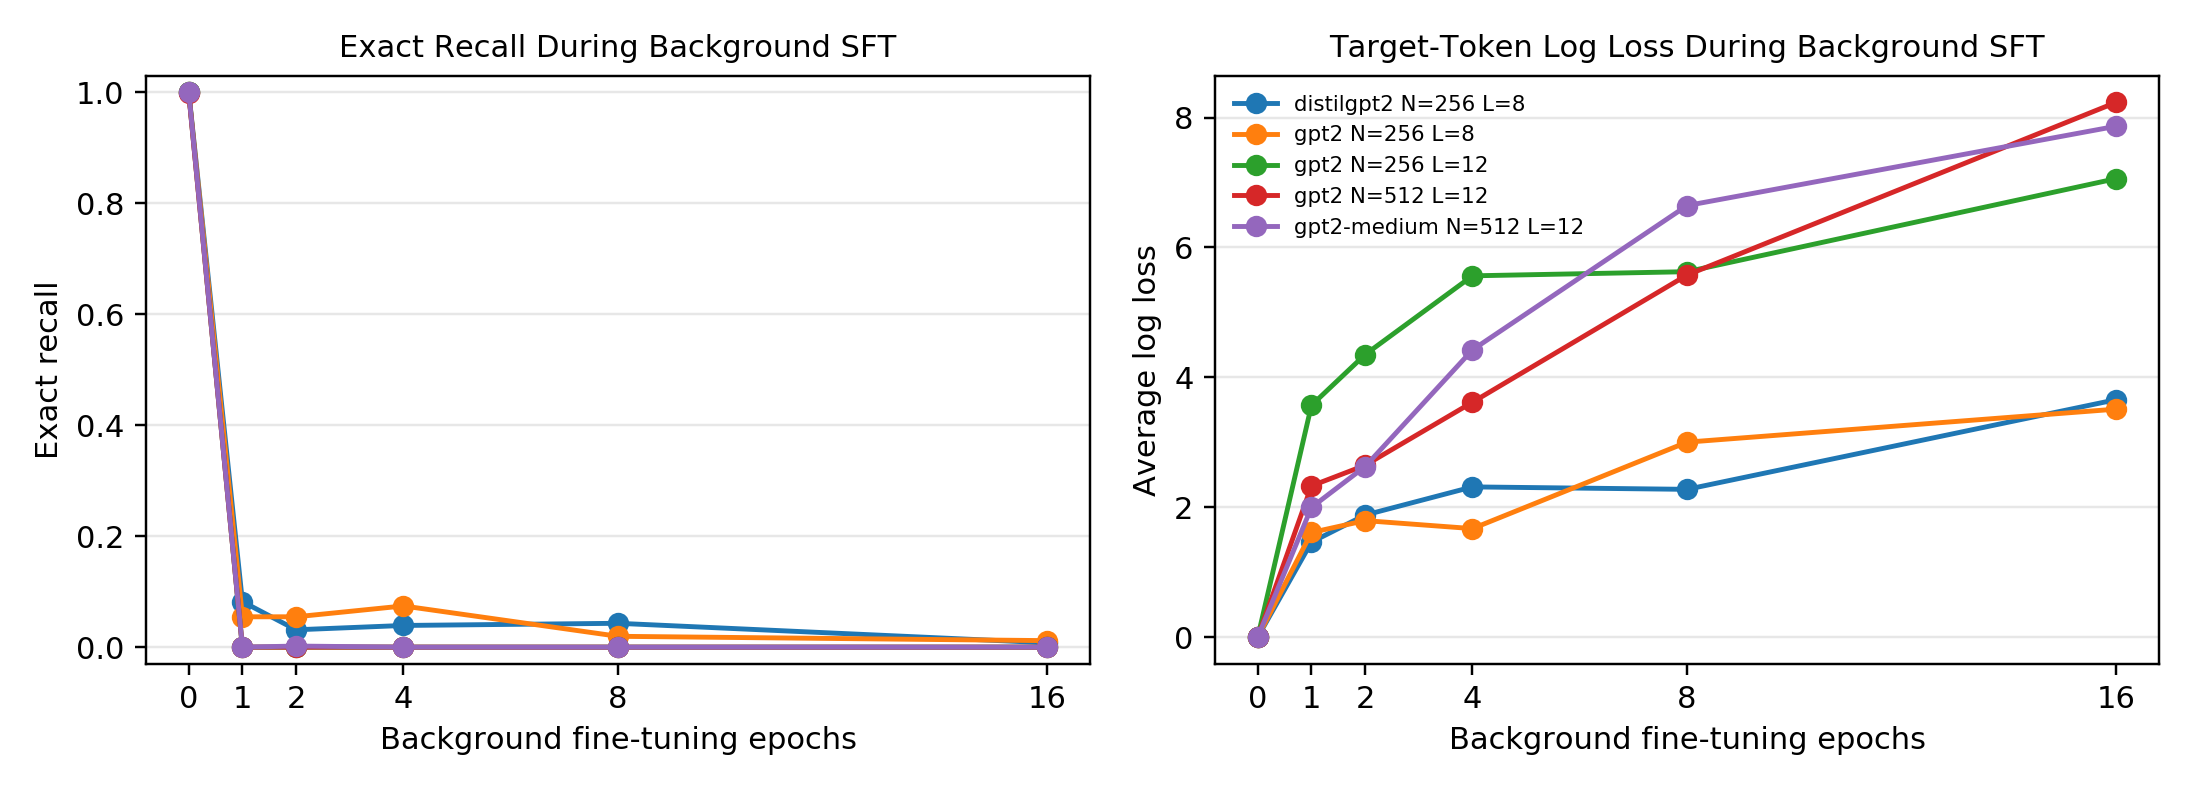
\includegraphics[width=\linewidth]{figures/scaled_recall_nll_curves.png}
\caption{Exact recall and target-token log loss over background fine-tuning epochs for representative scaled runs. Exact recall often reaches the floor quickly, while log loss continues to separate conditions after exact generation has collapsed.}
\label{fig:scaled-curves}
\end{figure}

\subsection{Claim C2: Load and Target Length}

To address C2 more directly, we compared completed \texttt{gpt2} runs that differ in target length at matched memorization load. Table~\ref{tab:h2-target-length} shows that 12-character targets are less stable than 8-character targets under the same model family. At $N=128$, the 8-character run retains 3/128 exact strings after one background epoch, while the 12-character run retains 0/128 and has higher log loss, 3.6297 versus 2.3433. At $N=256$, the 8-character run retains 14/256 after one epoch, while the 12-character run again retains 0/256 and has more than twice the one-epoch log loss.

\begin{table}[h]
\centering
\small
\caption{C2 target-length comparison for \texttt{gpt2}. All rows reach at least 0.996 exact recall before background fine-tuning. R is exact recall and NLL is average target-token log loss.}
\label{tab:h2-target-length}
\begin{tabular}{rrrrrrrr}
\toprule
$N$ & Len. & BG & Pre R & R@1 & NLL@1 & R@16 & NLL@16 \\
\midrule
128 & 8 & 1024 & 1.000 & 0.023 & 2.343 & 0.023 & 2.914 \\
128 & 12 & 1024 & 1.000 & 0.000 & 3.630 & 0.000 & 6.713 \\
256 & 8 & 2048 & 1.000 & 0.055 & 1.610 & 0.012 & 3.510 \\
256 & 12 & 2048 & 1.000 & 0.000 & 3.568 & 0.000 & 7.059 \\
\bottomrule
\end{tabular}
\end{table}

\begin{figure}[h]
\centering
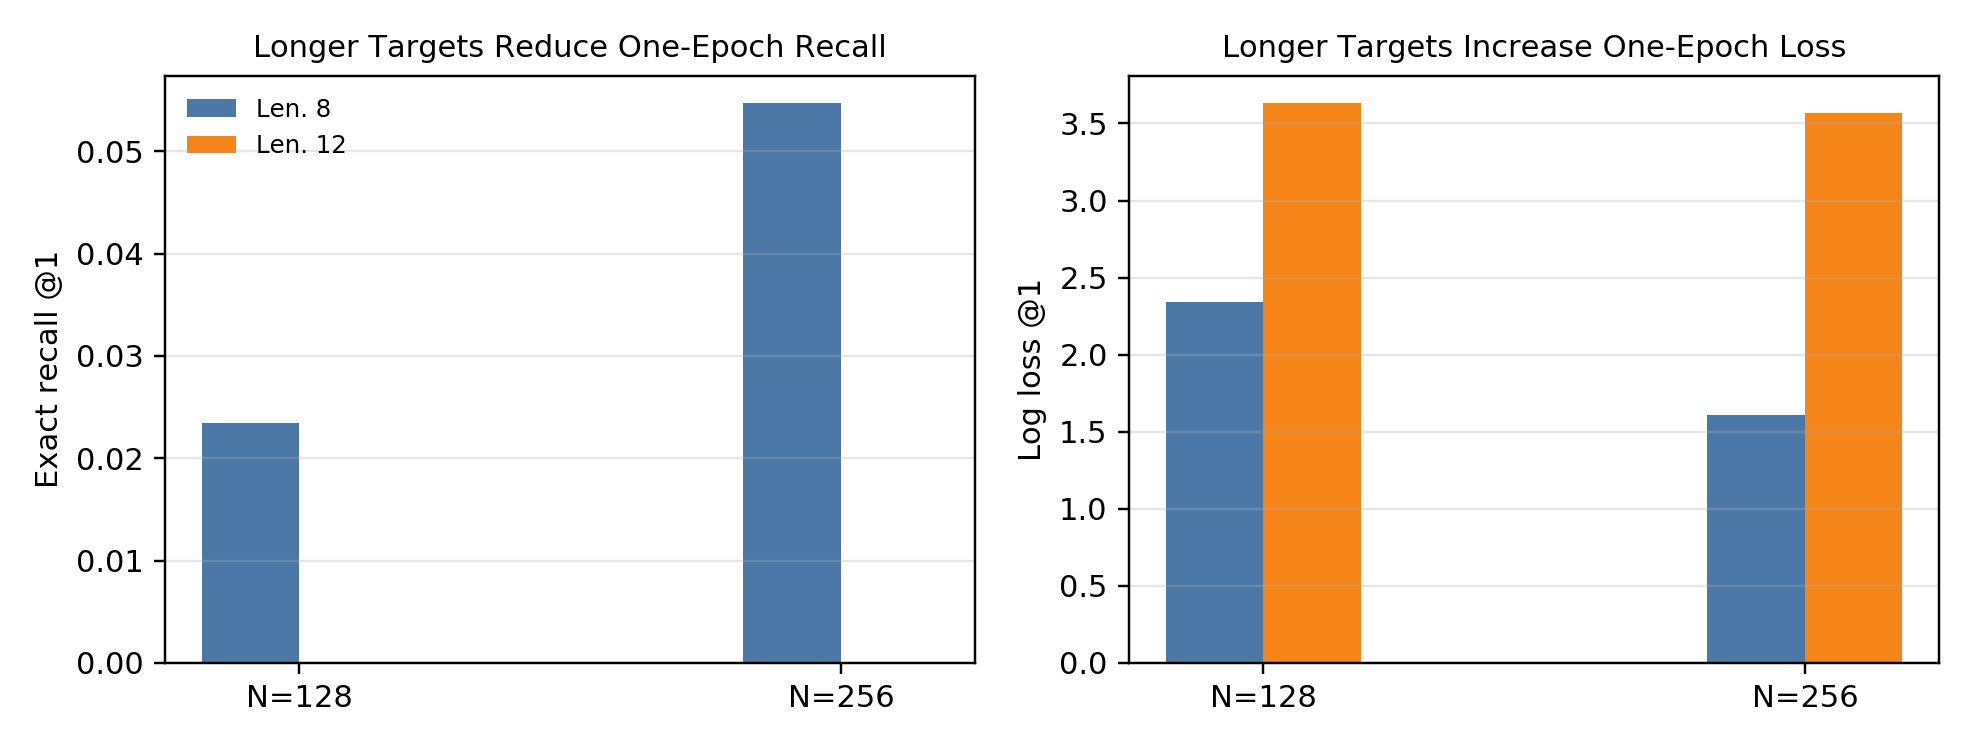
\includegraphics[width=0.95\linewidth]{figures/h2_target_length.png}
\caption{Target-length effect for matched \texttt{gpt2} loads. Longer 12-character targets have zero exact recall after one background epoch at both loads and substantially higher teacher-forced log loss.}
\label{fig:h2-target-length}
\end{figure}

The load effect is less cleanly isolated because the sweep increases background-set size together with memorization load. Still, the 12-character \texttt{gpt2} sequence becomes harder by the end of background training: NLL@16 is 6.713 for $N=128$, 7.059 for $N=256$, and 8.235 for $N=512$. This supports the target-length part of C2 and leaves the load component as suggestive rather than causal.

\subsection{Calibrating Forgetting Strength}

The first scaled sweep answered whether forgetting occurs, but it was too aggressive for detailed retention analysis: many runs reached zero exact recall after one background epoch. To make later checkpoints meaningful, we reused the memorized \texttt{gpt2-medium} checkpoint from the 512-key, 12-character run and varied only the second-stage background learning rate and background-set size. This isolates interference strength while holding the initial memorized state fixed at 512/512 exact recall.

\begin{table}[h]
\centering
\scriptsize
\caption{Forgetting-calibration results from the same memorized \texttt{gpt2-medium} checkpoint. All rows use 512 memorized examples with 12-character targets. $R$ is exact recall and NLL is average target-token log loss. LR is the background fine-tuning learning rate.}
\label{tab:calibrated-forgetting}
\setlength{\tabcolsep}{2.5pt}
\begin{tabular}{lrrrrrrrrrr}
\toprule
Setting & BG & LR & R@1 & R@2 & R@4 & R@8 & NLL@1 & NLL@2 & NLL@4 & NLL@8 \\
\midrule
Low LR, full BG & 4096 & $2{\times}10^{-6}$ & 0.945 & 0.807 & 0.410 & 0.098 & 0.018 & 0.065 & 0.300 & 0.854 \\
Very low LR, full BG & 4096 & $5{\times}10^{-7}$ & 1.000 & 0.990 & 0.961 & 0.867 & 0.001 & 0.003 & 0.012 & 0.045 \\
Base LR, small BG & 1024 & $2{\times}10^{-5}$ & 0.125 & 0.016 & 0.021 & 0.014 & 0.709 & 1.416 & 1.413 & 2.081 \\
Low LR, small BG & 1024 & $2{\times}10^{-6}$ & 1.000 & 0.988 & 0.951 & 0.869 & 0.001 & 0.004 & 0.014 & 0.048 \\
\bottomrule
\end{tabular}
\end{table}

Table~\ref{tab:calibrated-forgetting} shows that learning rate is the most important knob for avoiding floor effects. Reducing the background set from 4096 to 1024 examples is not enough by itself: at the original $2 \times 10^{-5}$ learning rate, recall still falls from 512/512 to 64/512 after one epoch and remains near zero. In contrast, $2 \times 10^{-6}$ with the full 4096-example background set gives a smooth decay from 512/512 to 484/512, 413/512, 210/512, and 50/512. This is the best calibrated configuration in the current sweep because it produces substantial forgetting while preserving enough signal to compare retention rates.

The log-loss values make the calibration difference visible even when exact recall remains high. With the full 4096-example background set, the $5 \times 10^{-7}$ run reaches only 0.0452 log loss after eight epochs while retaining 444/512 exact strings. The $2 \times 10^{-6}$ run reaches 0.8538 log loss and retains 50/512 strings.

The combined recall and log-loss view separates abrupt from gradual forgetting. The base-learning-rate, small-background run is nearly unrecoverable after one epoch, while the low-learning-rate, full-background run moves from 0.945 recall and 0.0176 log loss after one epoch to 0.098 recall and 0.8538 log loss after eight epochs. Useful retention experiments should target this intermediate regime before exact generation completely collapses.

\begin{figure}[h]
\centering
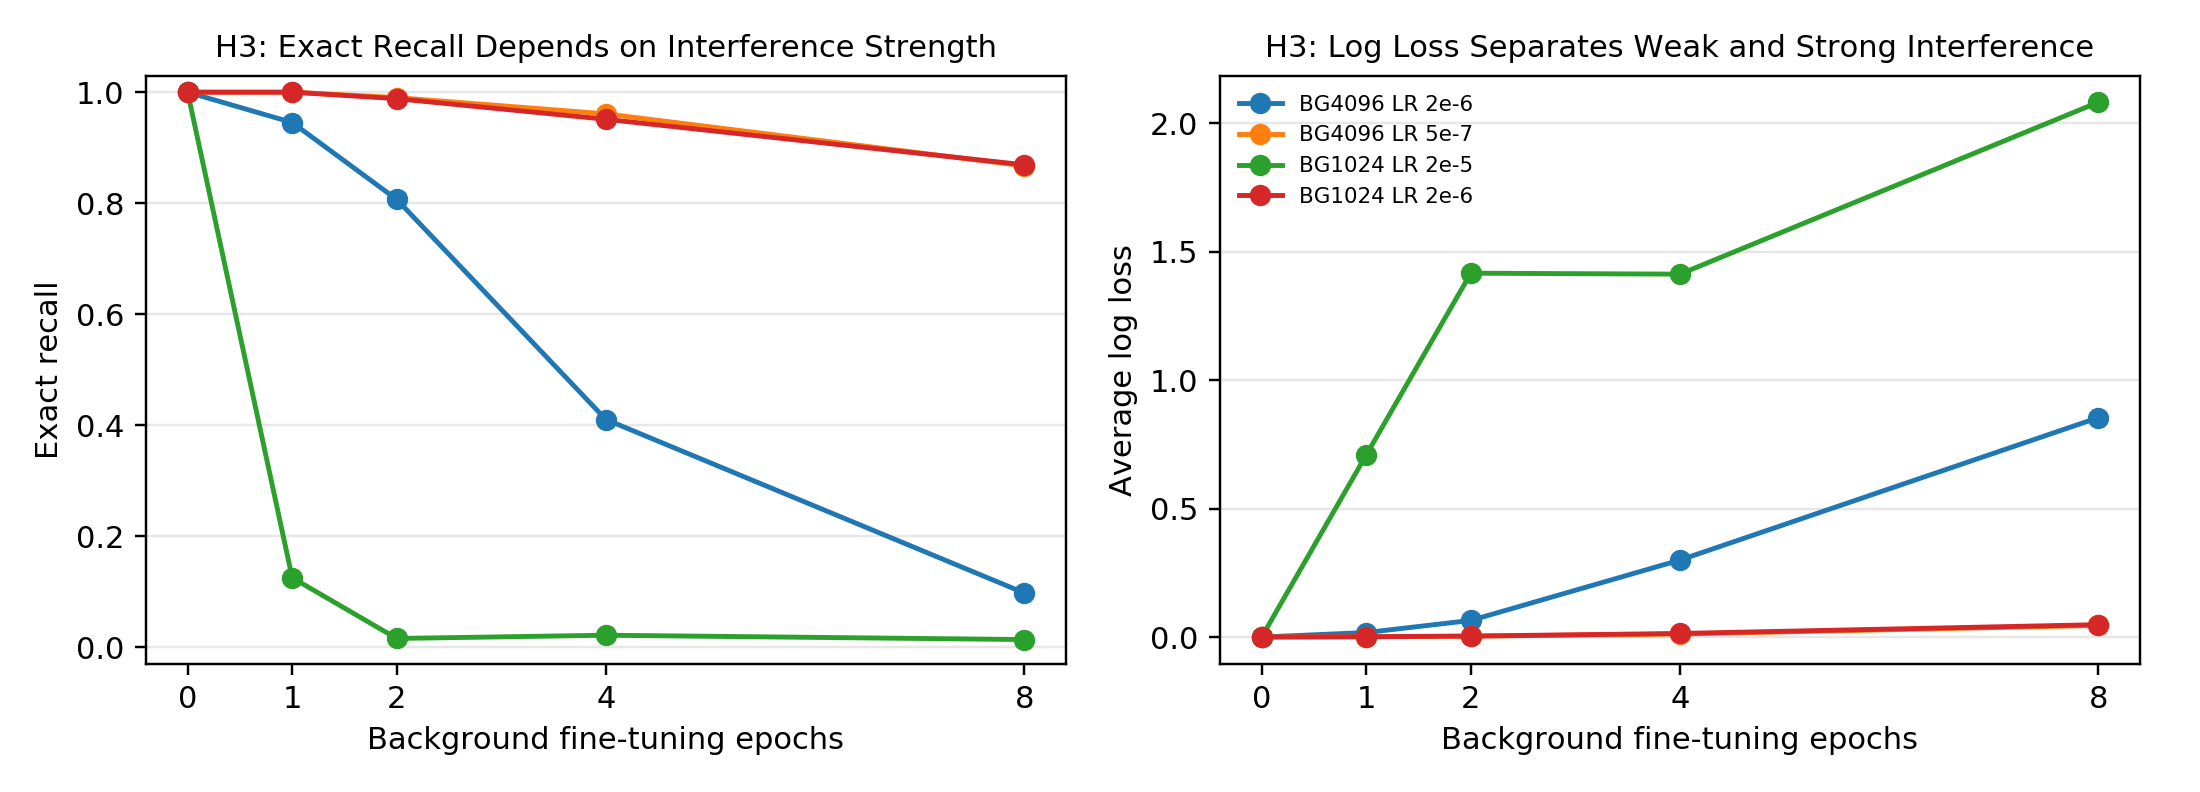
\includegraphics[width=\linewidth]{figures/h3_calibration_curves.png}
\caption{C3 calibration curves from the same memorized \texttt{gpt2-medium} checkpoint. Changing background learning rate and background-set size changes both exact retention and teacher-forced confidence, even though the pre-forgetting memorized state is fixed.}
\label{fig:h3-calibration}
\end{figure}

\subsection{Interpretation of Exact Recall}

Exact recall is a strict and somewhat brittle metric. In the \texttt{gpt2} 128-key, 8-character run, recall is 3/128 after one background epoch, 0/128 after two epochs, 5/128 after four epochs, 14/128 after eight epochs, and 3/128 after sixteen epochs. This non-monotonicity should not be read as steady relearning; it reflects the sensitivity of greedy generation to small probability changes. Teacher-forced log loss is therefore a better signal of gradual confidence decay, while exact recall remains the privacy-relevant recoverability metric.

The scaled sweep shows the same distinction. Several settings have identical zero exact recall at the first and last background checkpoints, but their log losses reveal different depths of forgetting. For example, the 512-key \texttt{gpt2} run moves from NLL 2.3275 at one epoch to 8.2346 at sixteen epochs, while the 512-key \texttt{gpt2-medium} run moves from 1.9965 to 7.8661. Exact recovery is already gone in both cases, but the teacher-forced metric shows that the original secrets continue to lose probability mass as background training proceeds.

\subsection{Capacity and Prompt Format}

The tiny-model controls did not produce meaningful memorization. These runs do not test forgetting because there was no successful memorized state to forget, but they are still informative negative controls: they show why a pre-forgetting recall gate is necessary before interpreting any retention curve.

The scaled runs show that larger GPT-2-family models can memorize substantially larger keyed datasets than the local calibration, but they do not show that capacity alone protects memorized strings under the original background setup. At 512 memorized 12-character strings, both \texttt{gpt2} and \texttt{gpt2-medium} reach essentially perfect pre-forgetting recall and fall to zero exact recall after one background epoch. The calibration sweep gives a stronger result for C3: background learning rate and effective interference strength substantially affect the stability budget.

\section{Discussion}

The main conclusion is that memorized random strings can be fragile under later fine-tuning, but measuring this effect requires both successful initial memorization and an interference regime that is not immediately saturated. The local calibration showed recall falling from perfect recovery to one quarter recovery; the scaled GPU reruns reproduced the pattern at larger memorization loads. The target-length analysis supports C2 by showing that 12-character targets are less stable than 8-character targets at matched \texttt{gpt2} loads. The calibrated forgetting sweep supports C3 by showing that lowering the background learning rate can turn a floor effect into a usable retention curve. Overall, the evidence is strongest for C1 and C3, with a narrower but clear result for target length in C2.

The sweep should not be overinterpreted as a full scaling law because several factors vary at once and the original background SFT setup often collapses recall by the first checkpoint. The calibration results show that this is a tunable measurement problem rather than a binary property of the model: at $2 \times 10^{-6}$, the same \texttt{gpt2-medium} checkpoint yields a comparable sequence of retention values across 1, 2, 4, and 8 background epochs.

The deeper pattern is that recoverability and residual confidence are related but not interchangeable. Exact recall asks whether a simple generation procedure can recover the full string. Log loss asks whether the model still assigns unusually high probability to the true string under teacher forcing. In a privacy setting, exact recall is the direct leakage event, while log loss is an early-warning signal: a model can stop emitting a secret before the association has been fully erased from its conditional distribution.

\subsection{What was Easy}
The synthetic setup made the core workflow manageable without making the experiment trivial. Random alphanumeric targets gave unambiguous ground truth, background tasks required no external data, and target-only loss aligned the training objective with the memorization question. Separate scripts for data generation, training, evaluation, and aggregation made reruns and error analysis straightforward.

\subsection{What was Difficult}
The main difficulty was finding regimes that both memorize and forget measurably. Tiny models were useful for debugging but did not memorize enough to support retention analysis, while the first GPU sweep forgot so quickly that many curves hit the floor after one checkpoint. The later calibration sweep fixed this by lowering the background learning rate. Compute also limited breadth: repeated seeds would improve reliability, but should wait until the larger GPT-2-family runs are more efficient.

\subsection{Recommendations for Future Work}
Future work should require a pre-forgetting recall threshold, such as $R(0) \geq 0.9$, before launching background fine-tuning. The next step is to add earlier interference checkpoints, such as fractions of one background epoch or fixed optimizer-step intervals, because much of the recall loss happens before the first full-epoch checkpoint.

The most useful extension is to vary one factor at a time, such as memorization load, target length, background learning rate, or background dataset size, while keeping model and optimizer fixed. The current calibration suggests that $2 \times 10^{-6}$ is a good starting background learning rate for 512-key \texttt{gpt2-medium} retention curves, while $5 \times 10^{-7}$ is a weak-interference control and $2 \times 10^{-5}$ is too strong for epoch-level comparison. Future runs should keep keyed prompts, add earlier step-level checkpoints, repeat calibrated settings across seeds, and report exact recall, teacher-forced log probability, and average log loss.


\bibliographystyle{plainnat}
\bibliography{references}

\clearpage
\appendix
\section{Appendix: Reproducibility and Validity Details}

\subsection{Code Availability}
The project repository is available at \url{https://github.com/yuewu7677/AML-project.git}.

\subsection{Reproducibility Checklist}
All experiments use synthetic datasets generated from a fixed seed, with memorization examples and background examples written as JSONL files. The codebase separates data generation, memorization fine-tuning, background fine-tuning, evaluation, aggregation, and plotting. The main scripts are:
\begin{itemize}[leftmargin=*]
    \item \path{scripts/generate_datasets.py}
    \item \path{scripts/run_pipeline.py}
    \item \path{scripts/run_forget_from_checkpoint.py}
    \item \path{scripts/eval_recall.py}
    \item \path{scripts/aggregate_results.py}
    \item \path{scripts/plot_report_figures.py}
\end{itemize}
The aggregate table used by the report is \path{results/hyak/aggregate.csv}.

\begin{table}[h]
\centering
\small
\caption{Main experimental knobs used across the reported runs.}
\label{tab:appendix-config}
\begin{tabular}{ll}
\toprule
Component & Setting \\
\midrule
Models & \texttt{distilgpt2}, \texttt{gpt2}, \texttt{gpt2-medium}; tiny model for smoke tests \\
Memorization load & 16 local calibration; 128, 256, 512 scaled runs \\
Target strings & Unique random alphanumeric strings, length 6, 8, or 12 \\
Background data & Independently generated synthetic tasks, 128--4096 examples \\
Evaluation checkpoints & Before background SFT; after 1, 2, 4, 8, and 16 background epochs \\
Primary metrics & Exact greedy-generation recall; teacher-forced log probability; NLL \\
Default seed & 42 for dataset generation and training scripts unless otherwise specified \\
\bottomrule
\end{tabular}
\end{table}

\subsection{Claim Boundaries}
The main empirical claim is about sequential fine-tuning of small and medium GPT-2-family causal language models on synthetic prompt-secret data. The work does not claim a universal scaling law for all model sizes or training recipes. It also does not claim that a secret is fully erased when exact recall reaches zero; the likelihood results show that residual probability mass can remain after greedy generation stops recovering the full string.

The strongest evidence is for C1 and C3. C1 is supported by repeated collapse of exact recall after background SFT in runs that first achieved near-perfect memorization. C3 is supported by the forgetting-calibration sweep from the same \texttt{gpt2-medium} checkpoint, where changing only the second-stage learning rate and background scale changes the retention curve. C2 is partially supported: target length is tested at matched \texttt{gpt2} loads, but the memorization-load comparison is confounded by background-set size.

\subsection{Threats to Validity}
The main internal validity risk is that several scaled conditions are single-seed runs, so exact recall fluctuations may reflect optimizer or data-order idiosyncrasies. The report mitigates this by emphasizing teacher-forced log loss and by treating non-monotone exact recall as a decoding artifact rather than as evidence of relearning. The main construct-validity risk is that synthetic random strings isolate memorization cleanly but do not capture semantic leakage, paraphrase leakage, or realistic user prompting. The main external-validity risk is model scale: the results show a controlled mechanism in GPT-2-family models, not a claim about all deployed language models.

Future conference-quality extensions should repeat the calibrated regimes across seeds, add step-level checkpoints before the first full background epoch, vary one factor at a time, and evaluate stronger extraction procedures beyond greedy decoding. Those additions would turn the current controlled measurement study into a more definitive statistical characterization of memorization stability.

\end{document}
